\documentclass[11pt]{article}
\usepackage[T1]{fontenc}
\usepackage{lmodern}
\usepackage[margin=0.92in]{geometry}
\usepackage{amsmath,amssymb,amsthm,mathtools,microtype}
\usepackage{tikz}
\usepackage[hidelinks]{hyperref}
\pdfinfoomitdate=1
\pdftrailerid{}
\pdfsuppressptexinfo=15
\hypersetup{pdftitle={A pointwise scalar-trace bound through past shell contact},
 pdfauthor={Ricardo Maldonado},pdfsubject={Working manuscript for author and specialist review}}
\newcommand{\dd}{\,\mathrm d}
\newcommand{\norm}[1]{\lVert #1\rVert}
\newcommand{\HH}{\mathcal H}
\newtheorem{proposition}{Proposition}
\newtheorem{premise}{Retained premise}
\title{A pointwise scalar-trace bound through past shell contact}
\author{Ricardo Maldonado\\Independent Researcher}
\date{4 November 2026\\[3pt]\small Working manuscript for author and specialist review}
\begin{document}
\maketitle
\begin{abstract}
For a registered compact first perturbation of a five-dimensional
Einstein--scalar shell, we bound the actual physical scalar coefficient
uniformly through its first possible past shell contact.
The normalized master obeys a dynamic boundary equation with a verified
positive boundary mass and spring. Its bulk and boundary time dependence
combine into a common scalar shift of a positive selfadjoint operator.
On the fixed interval $-3\ell\le t\le0$, $\ell=10^{-6}$, a complete
bulk-plus-boundary graph-energy estimate gives
$\norm{A_0Z}<417$ and $|w(t,0)|<2$. An exact boundary cancellation then
yields $|\Phi_1(t,\Omega)|<2.5\,10^8$ for the physical first scalar
variation, including its shell embedding.
This coarse upper bound controls an actual linear coefficient; it is not
a computed response profile, measured-unit prediction, or nonlinear
amplitude window. The operator realization, contact evolution, and qualitative
activation have earlier precedents, including retained project results.
The contribution is their explicit quantitative application to this
registered packet and its physical trace. No second-order past preparation
or remote incoming-state selection is supplied.
\end{abstract}

\section{The physical trace and the retained packet}
An energy bound for a bulk master does not automatically bound the physical
scalar on a shell. In this problem the physical trace differentiates the
longitudinal master normally, while the shell law contains a second time
derivative. The aim is an explicit pointwise bound for that trace through
contact, obtained by one additional graph-energy estimate.
The methods of positive forms, dynamic boundary evolution, and boundary
energy exchange are standard~\cite{zahn,marta}.
Earlier project capsules already give quantitative actual future
waveforms, including the same $\ell=10^{-6}$ packet~\cite{waveforms}.
The present coarse upper bound concerns its negative-time contact
interval; it is not a first quantitative amplitude result or an improved
forward waveform.

We retain the five-dimensional normalization and the one-copy outward laws
for two identical interiors:
\begin{equation}
\begin{gathered}
 S_{\rm bulk}=\int\left[\frac R2-\frac{|\nabla\phi|^2}{2}
                                      -V_{\rm b}(\phi)\right]\dd\mu_g,\\
 {\rm Ric}_{AB}=\partial_A\phi\,\partial_B\phi+\frac23V_{\rm b}g_{AB},
 \quad \Box_g\phi=V_{\rm b}',\quad
 K^{\rm out}_{\mu\nu}=\frac{\sigma}{6}\gamma_{\mu\nu},
 \quad n_{\rm out}\phi=-\frac{\sigma'}2 .
\end{gathered}
\end{equation}
The fixed model uses
\begin{equation}
\begin{aligned}
 S(\phi)&=1-\phi+\phi^3/3,&V_{\rm b}&=(S')^2/2-2S^2/3,\\
 \sigma&=2S+10^{-3}(1+c_\sigma\phi),&
 c_\sigma&=\frac{96714321425692}{161839258930731}.
\end{aligned}
\end{equation}
In particular $\sigma''=4\phi$. The spherical background is
\begin{equation}
 g_0=\dd y^2+\rho^2[-\dd t^2+\cosh^2t\,\kappa_{S^3}],
 \qquad \dd y=-\rho\dd z,\qquad a=\rho_y/\rho,\quad p=\phi_{0,y}\ne0 .
 \label{eq:bg}
\end{equation}
The shell is $z=0$; increasing $z$ points into the positive collar, away
from the shell. A subscript $b$ denotes the background shell value.

\begin{premise}
The actual regular static branch, its analytic shell enclosure, the selected
wide-collar enclosure, and the full first metric--scalar reconstruction
are retained inputs. Identification with the canonical and common-harmonic
first state uses the full one-jet and the retained gauge/uniqueness bridge.
These analytic premises are not reproved by byte authentication or finite
rational checks. No nonlinear past family is assumed to have the first
packet's support at all parameter orders.
\end{premise}

For $H(\Omega)=n_1^2-n_2^2$, the registered longitudinal perturbation is
$P=\mathsf V(t,z)H$. The retained reconstruction gives
\begin{equation}
 \Psi=P/\rho^2,\quad h_{yy}=-4\Psi,\quad h_{y\mu}=0,\quad
 h_{\mu\nu}=2\Psi g_{0,\mu\nu},\quad
 \delta\phi=-3P_y/(\rho^2p).
 \label{eq:reconstruction}
\end{equation}
In the copy-even straight-shell representative, the normal embedding is
fixed by the trace-free Israel row. The physical first scalar, with its
embedding included under the retained bridge, is
\begin{equation}
 \Phi_1(t,\Omega)=S_{\rm phys}(t)H(\Omega),\qquad
 S_{\rm phys}(t)=\frac{3\mathsf V_z(t,0)}{\rho_b^3p_b}.
 \label{eq:physical}
\end{equation}
This is an angular quadrupole, with $|H|\le1$ and mean zero.
It is not a scalar mean or a monopole volume coefficient.

Put
\begin{equation}
 C=\rho(3a+2p_y/p),\quad
 \alpha=(\rho/\rho_b)^{3/2}p/p_b>0,\quad
 \mathsf V=\alpha\cosh^{-3/2}t\,w,\quad \alpha_z/\alpha=-C/2.
\end{equation}
The actual normalized master data are
\begin{equation}
\begin{gathered}
 w(0,z)=q_\ell(z),\qquad w_t(0,z)=e^{-z}q_\ell(z),\qquad\ell=10^{-6},\\
 q_\ell(z)=
 \begin{cases}
 \exp\!\left(4-\dfrac{\ell^2}{(z-\ell)(2\ell-z)}\right),
                                  &\ell<z<2\ell,\\
 0,&\text{otherwise}.
 \end{cases}
\end{gathered}
\label{eq:packet}
\end{equation}
The nonzero first velocity is retained. It is not the velocity of a
second-response approximation.

\section{The actual dynamic shell row and positive coefficients}
The master and its homogeneous dynamic boundary law are
\begin{equation}
\begin{gathered}
 w_{tt}-w_{zz}+\mathcal W(t,z)w=0,\qquad
 -w_z+\mu_b w_{tt}+\beta(t)w=0\quad(z=0),\\
 \mu_b=\frac1{\rho_b B_b},\qquad
 B_b=\frac{p_{y,b}}{p_b}+\frac{\sigma_b''}{2},\qquad
 \beta(t)=\frac{C_b}{2}
       +\mu_b\left(\frac{35}{4}\operatorname{sech}^2t-\frac{25}{4}\right).
\end{gathered}
\label{eq:boundary}
\end{equation}
These equations and a finite-slab characteristic/boundary-ODE construction
already occur in the retained physical-response record~\cite{response}.
The regular-cone capsule also gives the equivalent Wentzell law and its
normal convention~\cite{cone}. A tangential wave boundary equation and
bulk--boundary energy cancellation are standard, as in Zahn~\cite{zahn}.
The present task requires the signs of the \emph{actual} coefficients.

Write $\eta=\phi_0-1$ and $h=V_{\rm b}'/p$.
The static ODE and $\sigma''=4\phi$ give
\begin{equation}
 B_b=h_b-4a_b+2\phi_b,\qquad C_b/2=\rho_b(h_b-5a_b/2).
\end{equation}
Direct rational evaluation on the selected analytic shell box yields
\begin{equation}
 \frac1{1000}<\mu_b<\frac1{400},\qquad
 189<C_b/2<300-\frac1{160},\qquad
 180<\beta(t)<300\quad(t\in\mathbb R).
 \label{eq:shellcaps}
\end{equation}
The last inequality follows from $0\le\operatorname{sech}^2t\le1$:
the temporal correction lies between $-25\mu_b/4$ and $5\mu_b/2$.
Positive boundary mass alone would not prove the spring's sign.

The previously verified positive collar $0\le z\le8\ell$ has
$129\le\rho\le131$, $-7/50000\le p\le-3/25000$, and
\begin{equation}
 \mathcal W=\rho^2\mathcal Q-\frac{35}{4}\tanh^2t,\qquad
 \mathcal Q=2h^2-10ah+\frac{35}{4}a^2-V_{\rm b}''-\frac{p^2}{6},
 \qquad \frac13<\mathcal Q<6.
 \label{eq:potential}
\end{equation}
The collar proof is retained from the precursor calculation~\cite{precursor}.
The explicit time dependence now gives, on that same collar for all real $t$,
\begin{equation}
 \mathcal W>\frac{129^2}{3}-\frac{35}{4}
         =\frac{22153}{4}>5500,\qquad
 \mathcal W<131^2\,6=102966<103000.
 \label{eq:potentialcaps}
\end{equation}
No evolved future-field error or five-mean operator cap is transferred
to negative time.

Set $x=t/\ell$, $r=z/\ell$, $U(x,r)=w(\ell x,\ell r)$ and $q(x)=U(x,0)$.
Then
\begin{equation}
\begin{gathered}
 U_{xx}-U_{rr}+\mathcal VU=0,\qquad
 -U_r+\Lambda q_{xx}+b(x)q=0,\\
 \Lambda=\mu_b/\ell,\quad b(x)=\ell\beta(\ell x),\quad
 1000<\Lambda<2500,\quad180\ell<b<300\ell,\quad
 5500\ell^2<\mathcal V<103000\ell^2 .
\end{gathered}
\label{eq:scaled}
\end{equation}
Here $U_r$ points into the collar. Its sign is kept explicit throughout.

\section{The existing form realization and the contact evolution}
\label{sec:operator}
The time dependence separates simultaneously in the bulk and shell:
\begin{equation}
\begin{aligned}
 \omega(x)&=-\frac{35}{4}\ell^2\tanh^2(\ell x),&
 \mathcal V(x,r)&=\mathcal V_0(r)+\omega(x),&
 \mathcal V_0&=\ell^2\rho^2\mathcal Q,\\
 b(x)&=b_0+\Lambda\omega(x),&
 b_0&=\ell[C_b/2+(5/2)\mu_b].
\end{aligned}
\label{eq:separation}
\end{equation}
Use the real mass space and its form domain
\begin{equation}
 \HH=L^2(0,\infty)\oplus\mathbb R,\quad
 \norm{(u,q)}_{\HH}^2=\int_0^\infty u^2\dd r+\Lambda q^2,\quad
 {\cal F}=\{(u,u(0)):u\in H^1(0,\infty)\}.
\end{equation}
General Hilbert vectors have independent components; trace identification
is imposed on $ {\cal F}$.
Thin boundary layers show density. Using the auxiliary extension defined
below, the positive form
\begin{equation}
 a_0[u]=\int_0^\infty(u_r^2+\mathcal V_0u^2)\dd r+b_0u(0)^2
 \label{eq:form}
\end{equation}
is closed: a Cauchy sequence in its form norm converges in bulk $H^1$,
and the limiting endpoint component is its trace.
The form representation gives a positive selfadjoint operator
\begin{equation}
\begin{gathered}
 D(A_0)=\{(u,u(0)):u\in H^2(0,\infty)\},\\
 A_0(u,q)=\left(-u_{rr}+\mathcal V_0u,\,
                   \frac{-u_r(0)+b_0q}{\Lambda}\right).
\end{gathered}
\label{eq:operator}
\end{equation}
There is no additional static Robin condition on $D(A_0)$.
For $D(A_0^2)$ the trace identity for $A_0(u,q)$ supplies the
next compatibility condition.

This construction is standard and already appears in the project's
spectral domain analysis~\cite{spectra}. Its earlier unscaled Liouville
operator has potential $V_L=\rho^2\mathcal Q-5/2$, endpoint mass $\mu_b$,
and endpoint coefficient $C_b/2$. Thus the present unscaled static
expression is that expression shifted by $(5/2)I$, including the spring
shift $(5/2)\mu_b$. The present scaling multiplies the operator by $\ell^2$
and the Hilbert norm squared by $1/\ell$.
The auxiliary cutoff below is not an identification with the old global
cone operator or its spectrum.

For the construction extend only $\mathcal V_0$ smoothly beyond $r=6$,
interpolating to $6000\ell^2$ for $r\ge7$. Its bounds remain
$5547\ell^2<\mathcal V_0<102966\ell^2$.
No physical background outside the actual collar is asserted.
Writing $Z=(U,q)$, the problem is exactly
\begin{equation}
 Z_{xx}+[A_0+\omega(x)I]Z=0.
 \label{eq:abstract}
\end{equation}
Let $\widehat Z(s)=Z(-s)$, $s=-x$, and $Q(r)=q_\ell(\ell r)$.
Its data are $Z_0=(Q,0)$ and
$Z_1=(-\ell e^{-\ell r}Q,0)$. Flatness on an open shell collar places
both in every power domain of $A_0$; every initial power has zero
endpoint component. Since $\omega$ is even, the wave-group formula is
\begin{equation}
\begin{aligned}
 \widehat Z(s)={}&\cos(s\sqrt{A_0})Z_0+
               A_0^{-1/2}\sin(s\sqrt{A_0})Z_1\\
 &-\int_0^s A_0^{-1/2}\sin((s-v)\sqrt{A_0})\,
                   \omega(v)\widehat Z(v)\dd v .
\end{aligned}
\label{eq:volterra}
\end{equation}
The sine propagator norm is at most $s-v$. On $0\le s\le3$ its
Volterra operator norm is bounded by
\begin{equation}
 \frac92\sup_{|x|\le3}|\omega(x)|
       \le\frac{2835}{8}\ell^4<1 .
 \label{eq:contraction}
\end{equation}
Its Neumann series gives a unique solution. Commutation with $A_0$
gives the same convergence in every power-domain graph norm.
The equation, smooth $\omega$, and one-dimensional elliptic regularity
give joint smoothness up to the dynamic boundary.
This uses standard linear machinery, not a numerical evolution or a
new nonlinear theorem.

\section{Boundary energy, support, and the finite past interval}
For a regular solution define the complete estimating energy
\begin{equation}
 E(x)=\frac12\int_0^\infty
       (U_x^2+U_r^2+\mathcal VU^2)\dd r
        +\frac{\Lambda}{2}q_x^2+\frac{b(x)}2q^2.
 \label{eq:energy}
\end{equation}
All summands are nonnegative. The bulk lower-endpoint flux is
$-q_xU_r(0)$. The actual law $U_r(0)=\Lambda q_{xx}+bq$ cancels it
against the derivatives of \emph{both} boundary terms, leaving
\begin{equation}
 E'(x)=\frac12\int_0^\infty\mathcal V_xU^2\dd r
          +\frac{b_x}2q^2
       =\frac{d(x)}2\norm{Z(x)}_{\HH}^2,\qquad
 d(x)=-\frac{35}{2}\ell^3\operatorname{sech}^2(\ell x)\tanh(\ell x).
 \label{eq:energyidentity}
\end{equation}
Here $b_x=\Lambda d$ and $d\ge0$ for $x\le0$.
Consequently $E(x)\le E(0)$ toward the past.
This is not damping: the sign follows from the explicit temporal potential.
For comparison, damped Wentzell energies also retain endpoint kinetic
terms, but their decay has a different cause~\cite{dahmani}.

Moving-cut energy identities give finite propagation. For backward time
$s=-x$, the temporal coefficients decrease.
The outer-cut flux at $r=2+s$ is
$-(U_s+U_r)^2/2-\mathcal VU^2/2\le0$.
Before $s=1$, the inner-cut flux at $r=1-s$ is
$-(U_s-U_r)^2/2-\mathcal VU^2/2\le0$, including the same cancelling
mass and spring at the shell. Both excluded regions have zero initial
energy, so
\begin{equation}
 \operatorname{supp}U(-s,\cdot)\subset
 \begin{cases}
 [1-s,2+s],&0\le s<1,\\
 [0,2+s],&1\le s\le3.
 \end{cases}
 \label{eq:support}
\end{equation}
The maximum depth is $r=5<6<8$; the auxiliary extension is irrelevant.
There is no claimed open shell gap after $s=1$. Smoothness and initial
flatness supply every differentiated initial corner condition.

\begin{figure}[htbp]
\centering
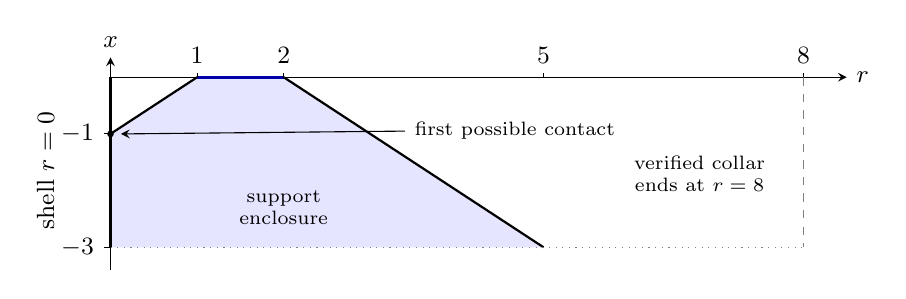
\begin{tikzpicture}[x=1.1cm,y=.72cm,>=stealth,font=\small]
 \fill[blue!10] (1,0)--(2,0)--(5,-3)--(0,-3)--(0,-1)--cycle;
 \draw[->] (0,0)--(8.5,0) node[right] {$r$};
 \draw[->] (0,-3.4)--(0,.35) node[above] {$x$};
 \draw[very thick] (0,0)--(0,-3);
 \draw[very thick,blue!65!black] (1,0)--(2,0);
 \draw[thick] (1,0)--(0,-1) (2,0)--(5,-3);
 \draw[gray,dashed] (8,0)--(8,-3);
 \draw[gray,dotted] (0,-3)--(8,-3);
 \foreach \r in {1,2,5,8} {
  \draw (\r,0)--(\r,.07) node[above] {$\r$};}
 \foreach \x in {-1,-3} {
  \draw (0,\x)--(-.08,\x) node[left] {$\x$};}
 \fill (0,-1) circle (1.2pt);
 \node[rotate=90] at (-.75,-1.65) {shell $r=0$};
 \node[font=\scriptsize,align=center] at (2.0,-2.3) {support\\enclosure};
 \node[font=\scriptsize,align=center] at (6.8,-1.7) {verified collar\\ends at $r=8$};
 \draw[->] (3.4,-.95)--(.12,-1);
 \node[font=\scriptsize,anchor=west] at (3.4,-.95) {first possible contact};
\end{tikzpicture}
\caption{The first-master support enclosure on $-3\le x\le0$.
Shading bounds possible support, not wave amplitude.
The boundary law is retained after the front reaches the shell at $x=-1$;
the whole support remains inside the verified collar.}
\label{fig:support}
\end{figure}

Positivity also gives
$E\ge(5500\ell^2/2)\norm{Z}_{\HH}^2$, since
$b/\Lambda>180\ell/2500>5500\ell^2$. Integrating
\eqref{eq:energyidentity} exactly yields
\begin{equation}
 (1-\epsilon)E(0)\le E(x)\le E(0),\qquad
 \epsilon=\frac{63\ell^2}{4400},\qquad -3\le x\le0.
 \label{eq:almost}
\end{equation}
Indeed $E(0)-E(x)\le[-\omega(x)/(5500\ell^2)]E(0)$ and
$|\tanh(\ell x)|\le3\ell$. The energy is a mathematical control norm
with time-dependent weights; it is not an identified physical Noether
or injected energy.

At $x=0$ the boundary terms vanish. If $D_Q=\norm{Q_r}_2$,
the endpoint Cauchy inequality $\norm{Q}_2\le D_Q/2$ gives
\begin{equation}
 \frac{D_Q^2}{2}\le E(0)\le
       \left[1+\frac{103001\ell^2}{4}\right]\frac{D_Q^2}{2}.
 \label{eq:initialenergy}
\end{equation}
For $q_p(s)=U(-s,0)$ the boundary mass and zero history for $s\le1$
give
\begin{equation}
 |q_p'(s)|^2\le E(0)/500,\qquad
 |q_p(s)|^2\le(s-1)_+^2E(0)/500\le E(0)/125 .
 \label{eq:q}
\end{equation}
This controls a master trace. A pointwise physical scalar bound needs
the additional estimate below.

\section{A graph-energy bound for the physical scalar}
\label{sec:graph}
The particular smooth packet has useful explicit derivative bounds.
For $1<r<2$ put $y=[(r-1)(2-r)]^{-1}\ge4$ and $a_*=3-2r$.
Then $|a_*|\le1$ and
\begin{equation}
 Q=e^{4-y},\qquad Q_r=a_*y^2Q,\qquad
 Q_{rr}=(a_*^2y^4-2a_*^2y^3-2y^2)Q.
 \label{eq:bumpderivatives}
\end{equation}
For $n=2,3,4$, the function $y^ne^{4-y}$ is nonincreasing for $y\ge4$.
Endpoint flatness and unit support length therefore give
\begin{equation}
 \norm{Q}_2\le1,\qquad \norm{Q_r}_2\le16,\qquad
 \norm{Q_{rr}}_2\le256+128+32=416.
 \label{eq:bumpnorms}
\end{equation}
These are analytic bounds, not new bump samples.

Let $Z^{[1]}=A_0^{1/2}Z$. The square root is nonlocal;
no compact-support assertion is made for this vector.
Power-domain regularity and scalar commutation nevertheless give
$Z^{[1]}_{xx}+(A_0+\omega I)Z^{[1]}=0$.
Its \emph{complete} mass-space/form energy obeys the abstract version of
\eqref{eq:energyidentity}, so $E_1(x)\le E_1(0)$ backwards.
Set $\kappa_0=5500\ell^2$. Coercivity gives $A_0\ge\kappa_0I$, and
$|\omega|/\kappa_0\le\epsilon$ on the slab. Hence
\begin{equation}
\begin{aligned}
 E_1(x)&=\frac12\norm{Z^{[1]}_x}_{\HH}^2
       +\frac12\norm{A_0Z}_{\HH}^2
       +\frac{\omega(x)}2\norm{A_0^{1/2}Z}_{\HH}^2\\
 &\ge\frac{1-\epsilon}{2}\norm{A_0Z}_{\HH}^2 .
\end{aligned}
\label{eq:graphcoercive}
\end{equation}
Every boundary contribution is retained in this identity.
One cannot set the boundary component of $Z^{[1]}$ to zero merely because
the original data have a shell gap.

At $x=0$, $\omega=0$. Write $f=-\ell e^{-\ell r}Q$.
Flatness gives $A_0Z_0=(-Q_{rr}+\mathcal V_0Q,0)$ and
\begin{equation}
\begin{aligned}
 2E_1(0)&=\norm{A_0Z_0}_{\HH}^2+a_0[f]\\
 &\le[416+103000\ell^2]^2
       +\ell^2[(16+\ell)^2+103000\ell^2].
\end{aligned}
\label{eq:graphinitial}
\end{equation}
The form equality
$\norm{A_0^{1/2}(f,0)}_{\HH}^2=a_0[f]$ includes all contributions of
the nonlocal square root. Exact rational comparison of
\eqref{eq:graphcoercive}--\eqref{eq:graphinitial} yields
\begin{equation}
 \norm{A_0Z(x)}_{\HH}<417,\qquad-3\le x\le0.
 \label{eq:417}
\end{equation}
Also \eqref{eq:bumpnorms} in the basic initial energy gives $E(0)<129$.
Equation~\eqref{eq:q} then gives $|q(x)|<2$ on the same slab.

The physical trace in \eqref{eq:physical} is not $q$.
Since $\alpha_b=1$ and $\alpha_{z,b}=-C_b/2$, the endpoint component
$(A_0Z)_b$ gives the exact cancellation
\begin{equation}
\begin{aligned}
 S_{\rm phys}(\ell x)
 =\frac{3\mu_b\cosh^{-3/2}(\ell x)}{\rho_b^3p_b}
       \left[-\frac{(A_0Z)_b}{\ell^2}+\frac52q\right].
\end{aligned}
\label{eq:traceidentity}
\end{equation}
Indeed $U_r=b_0q-\Lambda(A_0Z)_b$, so
$U_r/\ell-(C_b/2)q=\mu_b[-(A_0Z)_b/\ell^2+(5/2)q]$.
The temporal shift cancels. This controls the required normal derivative
without claiming a pointwise acceleration bound from the basic energy alone.
The mass norm implies
\begin{equation}
 \mu_b|(A_0Z)_b|\le\sqrt{\mu_b\ell}\norm{A_0Z}_{\HH},
 \qquad \sqrt{\mu_b\ell}<\frac1{20000}.
 \label{eq:boundarygraph}
\end{equation}
Using $\rho_b\ge129$, $|p_b|\ge3/25000$, and
$\cosh^{-3/2}t\le1$, we obtain
\begin{equation}
\begin{aligned}
 |S_{\rm phys}(t)|
 &<\frac{3}{129^3(3/25000)}
   \left[\frac{417}{20000\ell^2}
                    +\frac52\,\frac1{400}\,2\right]\\
 &<250000000,\qquad -3\ell\le t\le0 .
\end{aligned}
\label{eq:physicalbound}
\end{equation}
Because $|H|\le1$, the same upper bound holds for $|\Phi_1(t,\Omega)|$.
It is deliberately conservative and supplies no response profile or
numerical lower amplitude.

\section{Activation, clock interpretation, and scope}
The earlier physical-response record proves qualitative forward activation
for this actual packet~\cite{response}. The same zero-extension argument,
with the backward velocity sign retained, supplies the following limited
past statement. Suppose $S_{\rm phys}$ vanished on $(-T_1,0)$,
$\ell<T_1\le3\ell$. The original longitudinal boundary equation
\[
 \mathsf V_{tt}+3\tanh t\,\mathsf V_t
       +(8\operatorname{sech}^2t-4)\mathsf V
          =\rho_bB_b\mathsf V_z
\]
and zero initial shell value and velocity would force
$\mathsf V=\mathsf V_z=0$ there. Thus $w=w_z=0$ there.
Extending by zero to negative depth introduces no interface source.
Uniqueness identifies the extension with the auxiliary whole-line
Cauchy solution having backward velocity $-e^{-z}q_\ell(z)$.

Choose $0<\eta\le\min\{\ell/4,(T_1-\ell)/2\}$ and backward elapsed
time $S_{\rm obs}=\ell+\eta$.
Set $Q_{\rm front}=q_\ell(S_{\rm obs})>0$.
On the backward diamond of $(S_{\rm obs},0)$ only the increasing bump
edge is sampled, and the nonzero positive-depth portion of each source
slice has width at most $\eta$.
For $M=103000$ and $\beta_*=MS_{\rm obs}\eta/2$, Duhamel gives
\begin{equation}
 |w|_*\le\frac{Q_{\rm front}(1+\eta/2)}{1-\beta_*},\qquad
 w_{\rm aux}(S_{\rm obs},0)\ge
       \frac{Q_{\rm front}(1-\eta-3\beta_*)}{2(1-\beta_*)}>0.
\end{equation}
The guard holds since $\beta_*\le5M\ell^2/32$ and
$\eta+3\beta_*<1$. This contradicts the zero trace.
Therefore $S_{\rm phys}$ is nonzero somewhere in each
$(-T_1,-\ell)$ with $\ell<T_1\le3\ell$. It vanishes on $[-\ell,0]$,
and smooth flatness gives zero jets at the front itself.
The displayed positive auxiliary value is only a contradiction under the
zero-trace hypothesis. It is not a lower bound on the actual dynamic
response. In contrast, \eqref{eq:physicalbound} bounds the actual first
physical coefficient.

At the background proper shell clock $\tau=\rho_b t$, the background scalar
is constant. Consequently the first clock pullback adds no tangential
shift term or additional amplitude factor to
\eqref{eq:physical}--\eqref{eq:physicalbound}.
The result is a model-normalized first parameter derivative. It has no
SI calibration, does not estimate a finite-amplitude nonlinear deviation,
and supplies no effective uniform perturbation window.
The quadrupole has zero angular mean; this bound is not a monopole
shell-volume, heating, radiation-density, or particle-production estimate.

The earlier operator construction, dynamic law, and qualitative activation
are credited rather than claimed as new. The focused result is the
explicit graph-to-physical-trace bound for the registered packet on this
finite past interval. Even its estimating energy is not a physical
Noether or injected energy without an additional identification.
The precontact principal-channel shares must not be extrapolated through
reflection using energy alone.
Second-order bulk and junction sources, larger nonlinear correction
annuli and their contact times, a compatible nonlinear past family, and a
remote incoming preparation remain unsolved here. No observational signal
or cosmological origin is inferred.

\section{Verification and reproducibility}
The new standard-library arithmetic authenticates the selected local
shell box, precursor inputs, physical-response record, and prior spectral
domain note. It checks the actual boundary mass and spring signs,
scaling, temporal identities, graph majorants, and physical-trace cap
without a numerical PDE evolution, waveform evaluation, or new
background/source/bump oracle query.
The static branch, reconstruction, and gauge-identification premises
remain analytic inputs. The explicit fixed-form and wave-group argument
supplies the linear evolution, rather than a finite arithmetic claim
standing in for a PDE theorem.
The editable source, exact displayed-bounds audit, two fresh deterministic
three-pass PDF builds, all-page visual review, and independent
mathematical review accompany the working paper.

\begin{thebibliography}{9}
\bibitem{zahn}
J. Zahn, \emph{Generalized Wentzell boundary conditions and quantum field theory},
Ann. Henri Poincar\'e \textbf{19}, 163 (2018),
\href{https://arxiv.org/abs/1512.05512v3}{arXiv:1512.05512v3}.
Propositions 1--3 give the scalar operator, compatible evolution,
and bulk--boundary causal energy template.

\bibitem{marta}
A. Marta, \emph{The nonlinear wave equation with nonlinear Wentzell
boundary conditions on time-dependent compact Riemannian manifolds},
\href{https://arxiv.org/abs/2404.05855v2}{arXiv:2404.05855v2}.
The compact nonautonomous setting differs from this half-line problem.

\bibitem{dahmani}
A. Dahmani, Y. Chitour, H.-M. Nguyen, and C. Roman,
\emph{One dimensional wave equation with in-domain localized damping and
Wentzell boundary conditions},
\href{https://arxiv.org/abs/2503.22439v1}{arXiv:2503.22439v1}.
Section 4 retains dynamic endpoint energy; its decay uses damping.

\bibitem{spectra}
R. Maldonado, \emph{Regular shell spectra}, dated research capsule,
\href{https://github.com/maldonado-research/HDblast/tree/main/research/HDBLAST_REGULAR_SHELL_SPECTRA_20261013}{13 October 2026}.
The domain note, Sections 2--3 and 6, supplies the earlier endpoint-mass
realization and Liouville expression.

\bibitem{cone}
R. Maldonado, \emph{Regular cone evolution}, dated research capsule,
\href{https://github.com/maldonado-research/HDblast/tree/main/research/HDBLAST_REGULAR_CONE_EVOLUTION_20261013}{13 October 2026}.
The boundary note, Sections 2--4, fixes the Wentzell/Robin conversions.

\bibitem{response}
R. Maldonado, \emph{A nonzero physical scalar response in the conditional
exact shell family}, retained physical-response record,
\href{https://github.com/maldonado-research/HDblast/blob/main/research/HDBLAST_INTERIOR_MASTER_JETS_20261015/inputs/reference/PHYSICAL_SHELL_RESPONSE.md}{15 October 2026}.
Sections 2--3 contain the actual dynamic row, contact construction,
and qualitative activation argument.

\bibitem{precursor}
R. Maldonado, \emph{A local characteristic precursor for the registered
Einstein--scalar shell packet}, working manuscript,
\href{https://github.com/maldonado-research/HDblast/tree/main/research/HDBLAST_PAST_CHARACTERISTIC_PRECURSOR_20261105}{dated research capsule}.
Its UTC date identifier is retained unchanged.

\bibitem{waveforms}
R. Maldonado, \emph{Uniform first-variation waveform} and
\emph{A wider shell waveform with a certified signed inertial tail},
dated research capsules,
\href{https://github.com/maldonado-research/HDblast/tree/main/research/HDBLAST_UNIFORM_FIRST_VARIATION_WAVEFORM_20261015}{15 October 2026}
and
\href{https://github.com/maldonado-research/HDblast/tree/main/research/HDBLAST_INERTIAL_SHELL_WAVEFORM_20261015}{15 October 2026}.
The first uses $\ell=10^{-10}$; the latter uses the present
$\ell=10^{-6}$ and bounds the actual future physical trace.
\end{thebibliography}
\end{document}
